\documentclass[11pt]{article}
%\usepackage{fullpage,url}
\usepackage{url}
\usepackage{amsmath}
\usepackage{graphicx}
\usepackage{caption}
\usepackage{subcaption}

\usepackage[letterpaper,top=1in,bottom=1in,left=1in,right=1in,nohead]{geometry}

\setlength{\parindent}{0in}
\setlength{\parskip}{6pt}
\bibliographystyle{plain}

\DeclareMathOperator{\E}{E}
\DeclareMathOperator{\Var}{Var}
\DeclareMathOperator{\Unif}{Unif}
\DeclareMathOperator{\shrink}{shrink}

\begin{document}
\thispagestyle{empty}
{\large{\bf CS7640: Advanced Image Processing \hfill Danny Perry}}\\

{\LARGE{\bf Non-linear Image Denoising}}
\vspace{0.2\baselineskip}
\hrule

\section{Introduction}
One of the classic problems in image analysis is image denoising.
We are interested in the specific approaches to image denoising that preserve edges.
A classic approach to edge-preserving non-linear denoising was introduced by \cite{perona1990scale}, where edge preservation was achieved by modeling the problem as an anisotropic diffusion problem.
Later work in \cite{rudin1992nonlinear} introduced the so called "ROF Model" where edge-preserving denoising could be done my minimizing the total variation of the image.
Total variation minimization is based on the principle that noisy images have high total variation, which is the integral of the norm of the gradient.  
By reducing the total variation subject to being a close match to the original image removes unwanted detail (hopefully noise), while preserving important details like edges \cite{wikiTV}.

Here we evaluate three popular algorithms in minimization of total variation:
\begin{enumerate}
\item TV using Chambolle's Algorithm
\item TV using Primal-Dual Algorithm
\item Anisotropic TV using Split-Bregman Iterations
\end{enumerate}

\section{Methods}
Here we briefly describe the specific motivation for each algorithm, how they work in theory, and the specific engineering decisions used in the implementations.
\subsection{Total Variation Minimization}
Here we motivate and describe the method of total variation.
As briefly described above varation can be described like so:
\begin{equation*}
\int |\nabla u| dx dy
\end{equation*}
Where we want to minimize the varation while maintaining some similarity with the original image, we hope to minimize the following constrained problem:
\begin{equation}
\min \int |\nabla u| dx dy \text{ s.t.} \int (u-u_0)^2 dxdy = \sigma^2
\label{tv:isotropic}
\end{equation}
This specific formulation is referred to colloquially as the ROF model.
When originally presented in \cite{rudin1992nonlinear}, a gradient descent type algorithm was suggested to minimize the Euler-Lagrange equations of the problem.
While the results were good, the specific algorithm for solving it was numerically difficult, due to the possibility of $|\nabla u|=0$.
Later work, presented below attempted to improve on that approach.

\subsection{Chambolle's Algorithm}
In \cite{chambolle2004algorithm} a new formulation was presented introducing a so called "dual problem", which addressed the possible zero gradients by changing the formulation into a constrained maximization problem, ie
\begin{align*}
\int |\nabla u| dx xy &= \max_{|p| \le 1} \int p \nabla u dx dy \\
&= \max_{|p| \le 1} \int (\nabla \cdot p) u dx dy
\end{align*}
The second equation is obtained via integration by parts.  
In this form, the problem can be solved in a two-step approach:
\begin{enumerate}
\item
Gradient descent to maximize $p$:
\begin{equation}
p^{k+1} = p^{k} - \Delta t \left[ \nabla( \nabla \cdot p^{k}) + \lambda \nabla u_0 \right]
\label{ch:dual}
\end{equation}
\item Solution to the tv minimization:
\begin{equation}
u = f + \lambda \nabla \cdot \hat{p}
\label{ch:primal}
\end{equation}
\end{enumerate}
In practice this two step approach is repeated until desirable results are reached.

Here the implementation was done entirely in C++ using the ITK framework.
ITK was used primarily for image and vector data structures, I/O, and some infrastructure for parallelization.
Any actual numerics were rewritten for this project, including gradient and divergence operations.
A reader interested in following the code would be directed to primarily read the respective "GenerateData()" and "ThreadedGenerateData()" methods of the .hxx files of the classes described below, as that is where the action takes place - the rest is infrastructure. 
A README.txt file in the code directory describes how to build the executable.

In order to parallelize the algorithm, it was decomposed into a few distinct parallel steps over the image, with a single threaded iteration loop.  
The structure follows directly the algorithm structure:
\begin{enumerate}
\item
ChambolleFilter.h,.hxx - the main loop
\item
ChambolleDualFilter.h,.hxx - the parallel dual solution
\item
ChambollePrimalFilter.h,.hxx - the parallel primal solution \\
DivergenceFilter.h,.hxx - the parallel divergence computation \\
UnitGradientFilter.h,.hxx - the parallel unit gradient computation
\end{enumerate}

As discussed in class, I found it important to "balance" the one-sided derivatives used, so that the result ended up "on the grid" and not in the "gap".
For example, in this solution I use a "right-sided" difference for the gradient and a "left-sided" difference for the divergence.

The implementation was done primarily from in class notes, which some details taken from the original paper.

It's also worth noting that because of the double loop needed to obtain quality results, this algorithm is the slowest of the three algorithms investigated.
Specific results will be discussed below.

\subsection{Primal-Dual Algorithm}
A more efficient solution to the primal and dual problems called the Primal-Dual algorithm was described in \cite{zhu2008efficient}.
Instead of solving the dual problem to completion (\ref{ch:dual}) and then using that solution in the primal (\ref{ch:primal}), the Primal-Dual algorithm solves both problems simultaneously in a sort of combined gradient descent.

In a single main iteration two steps are used to find the solution to the primal and dual equations:
\begin{enumerate}
\item Dual step:
\begin{equation}
p^{k+1} = P_p(p^k + \tau_k \lambda A^T u^k)
\label{pd:dual}
\end{equation}
Where $P_p(z)$ is the projection back onto $p$.
\item Primal step:
\begin{equation}
u^{k+1} = u^k - \theta_k (1/\lambda Ap^{k+1} + u^k-u_0)
\label{pd:primal}
\end{equation}
\end{enumerate}

Again, this was implemented in a parallel fashion using C++ and ITK.
A single thread loop controlled the main iteration, while separate parallel processes compute each step.
Here is the specific break down:
\begin{enumerate}
\item PrimalDualFilter.h,.hxx - the main loop
\item DualFilter.h,.hxx - the parallel dual step
\item PrimalFilter.h,.hxx - the parallel primal step\\
UnitGradientFilter.h,.hxx - parallel unit gradient computation
\end{enumerate}

Again, the "balance" of the derivatives was very important here.
Similar to above the gradient used a "right-sided" difference, while the divergence was computed using a "left-sided" difference.

While I found it necessary to compute the initial $p$ unit gradient field, all other gradient and divergence calculations are done in the dual and primal step filters themselves.

I primarily used the original paper to do the implementation.

This algorithm was much faster than Chambolle's, but specific results are shown below.

\subsection{Split-Bregman Algorithm}
The most recent of those approaches discussed here, is the Split-Bregman approach described in \cite{goldstein2009split}.  
While the two methods discussed above are quite similar, this approach takes a slightly different route.
Also, while the above algorithms minimize isotropic total variation, the algorithm implemented here minimizes an anisotropic total variation.
The same paper \cite{goldstein2009split} describes an isotropic version of Split-Bregman, but is not discussed in this report.

Instead of solving the problem described in \ref{tv:isotropic}, the anisotropic Split-Bregman addresses this similar anisotropic problem:
\begin{equation}
\arg \min_{u}\left[ |du/dx|_1 + |du/dy|_1 + \frac{\mu}{2}||u-u_o||^2_2 \right]
\label{tv:anisotropic}
\end{equation}

The basic algorithm is as follows:
\begin{enumerate}
\item A single Gauss-Seidel (or similar) step to solve the $L_2$ problem.
\begin{equation*}
u^{k+1} = G(u^k,d^k,b^k)
\end{equation*}
\item A shrinkage step
\begin{equation*}
d^{k+1}_x = \shrink(\nabla_x u^{k+1} + b^k_x, 1/\lambda)
\end{equation*}
\begin{equation*}
d^{k+1}_y = \shrink(\nabla_y u^{k+1} + b^k_y, 1/\lambda)
\end{equation*}
\item A Bregman update
\begin{equation*}
b^{k+1}_x = b^k_x + (\nabla_x u^{k+1} - d^{k+1}_x)
\end{equation*}
\begin{equation*}
b^{k+1}_y = b^k_y + (\nabla_y u^{k+1} - d^{k+1}_y)
\end{equation*}

\end{enumerate}

This was also implemented in C++ using ITK.
This algorithm was surprisingly simple to implement.
It's the only algorithm where I simply coded up the algorithm, compiled, and it worked.
This may have been due to it being the last one implemented, but I'd like to think it's somewhat due to the simplicity and robustness of the approach.
It was also surprising how fast it is.  
When I first completed the code I thought something must be wrong, but it just converges very quickly.

To parallelize this code, I broke the algorithm into two distinct parallel steps, the Gauss-Seidel step and a combined shrinkage and Bregman update step, with a single iteration loop:

\begin{enumerate}
\item SplitBregman.h,.hxx - the main loop
\item GaussSeidelFilter.h,.hxx - the parallel Gauss-Seidel step
\item ShrinkBregmanFilter.h,.hxx - the parallel Shrink and Bregman update step
GradientFilter.h,.hxx - a parallel gradient filter
\end{enumerate}

This code was mainly implemented using the original paper \cite{goldstein2009split}, however a few details like edge conditions, etc. I obtained from Goldsteins implementation available for download at his website \cite{goldsteinImplementation}.

\section{Results}

Each algorithm was run against several images.  
The results of three of those images are show below: the cameara man image (Figures \ref{fig:cameraman:dn},\ref{fig:cameraman:diff}), a sailboat image (Figures \ref{fig:sailboat:dn},\ref{fig:sailboat:diff}), and a slice of a seismic image (Figure \ref{fig:slice:dn}).

For the cameraman and sailboat images Gaussian noise with $\sigma^2=100$ was added to the image.
This was done to make the denoising effect more apparent.

For the slice of seismic volume, the image was equalized to bring out the horizons.
Denoising was applied with the goal of making the horizons appear more continuous.
The seismic image is a slice taken from the Netherlands data set found on the OpendTect data repository \cite{opendTectWeb}.

\subsection{Chambolle's Algorithm}

Chambolle's algorithm was the slowest of the algorithms by far - mostly due to it's use of two loops.  
The bar graph in Figure \ref{fig:timing} details the speed comparison.
While Primal-Dual and Split-Bregman were comparable, both performed much faster than Chambolle.

As mentioned before, Chambolle's main cost are the double loops.
The inner loop would normally take about 200-300 iterations to converge for the first few outer loop iterations, then it would take only a few iterations (under 10) to converge for the remaining outer loop iterations.
Convergence criteria of the inner loop was computed using the difference of result with the previous - when the result started converging less than an epsilon, the loop was terminated.

The outer loop would converge in about 10-20 iterations.
Visual correctness was used to determine convergence of the outer loop.
The resulting total iterations required usually came to about 1000 iterations, which is the big reason for Chambolle's poor speed.


The quality of Chambolle's algorithm is good.  
It would be difficult to argue whether the results are much better or worse than from the other algorithms. 
For example Figures \ref{sail:ch},\ref{sail:ch:diff} show the result and difference from noisy image of Chambolle's method.  As you can see the result looks good and the difference image isn't obviously better than the other difference images.

Numerically, Chambolle was the trickiest to get right.
With certain step sizes, it is quite easy for Chambolle's algorithm to blow up and not converge.

For these experiments I chose a $\lambda=0.248$ as recommended in the Primal-Dual paper \cite{zhu2008efficient}.
I also used an initial dual step size of $\Delta t = 0.0001$, but then updated that step size each iteration as described below.
The dual step size was chosen proportional to the maximum gradient of the divergence of $p$, as indicated in class.
In other words, take the maximum:
\begin{equation*}
\max q = |\nabla(\nabla \cdot p) + \lambda \nabla u_0|
\end{equation*}
Then the step size was:
\begin{equation*}
\Delta t = \frac{1}{2q}
\end{equation*}



\begin{figure}
\centering
\graphicspath{{images/}}
\begin{subfigure}[b]{0.4\textwidth}
\centering
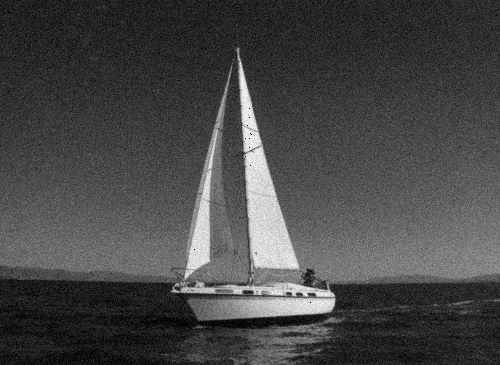
\includegraphics[width=\textwidth]{sailboat_10}
\caption{Noisy}
\label{sail:noise}
\end{subfigure}
\begin{subfigure}[b]{0.4\textwidth}
\centering
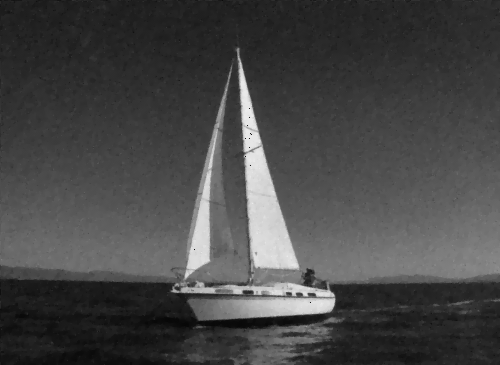
\includegraphics[width=\textwidth]{sailboat_10_ch}
\caption{Chambolle's}
\label{sail:ch}
\end{subfigure}
\begin{subfigure}[b]{0.4\textwidth}
\centering
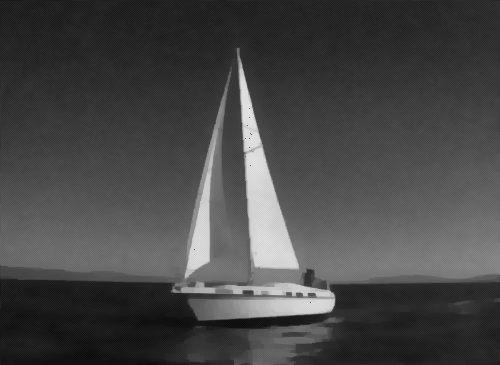
\includegraphics[width=\textwidth]{sailboat_10_pd}
\caption{Primal-Dual}
\label{sail:pd}
\end{subfigure}
\begin{subfigure}[b]{0.4\textwidth}
\centering
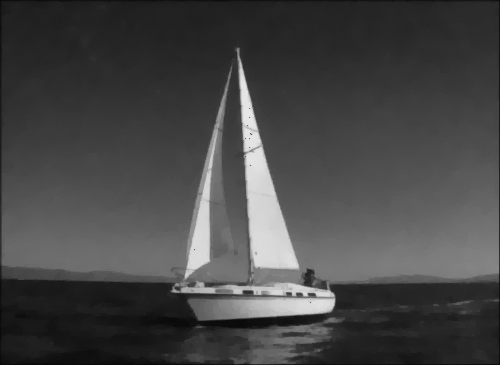
\includegraphics[width=\textwidth]{sailboat_10_sb}
\caption{Split-Bregman}
\label{sail:sb}
\end{subfigure}
\caption{Results of each algorithm on a noisy image of a sailboat.}
\label{fig:sailboat:dn}
\end{figure}

\begin{figure}
\centering
\graphicspath{{images/}}
\begin{subfigure}[b]{0.4\textwidth}
\centering
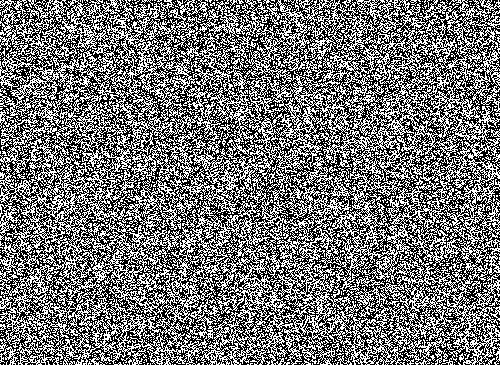
\includegraphics[width=\textwidth]{sail_gauss_diff}
\caption{Gaussian blur}
\label{sail:gauss:diff}
\end{subfigure}
\begin{subfigure}[b]{0.4\textwidth}
\centering
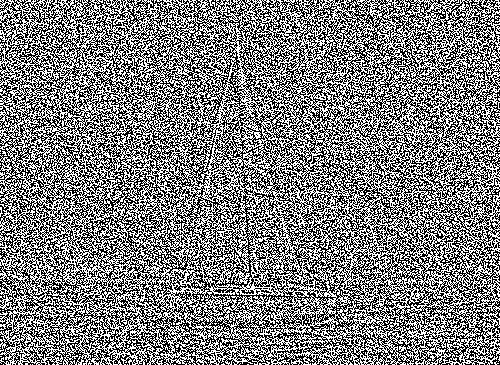
\includegraphics[width=\textwidth]{sail_ch_diff}
\caption{Chambolle's}
\label{sail:ch:diff}
\end{subfigure}
\begin{subfigure}[b]{0.4\textwidth}
\centering
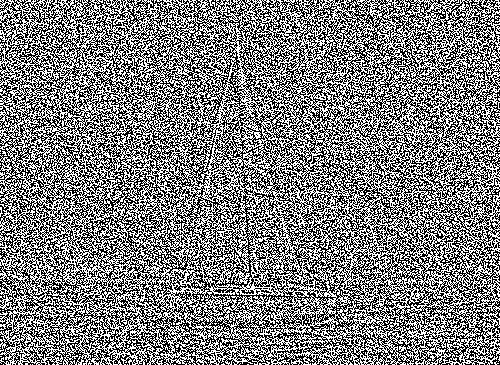
\includegraphics[width=\textwidth]{sail_pd_diff}
\caption{Primal-Dual}
\label{sail:pd:diff}
\end{subfigure}
\begin{subfigure}[b]{0.4\textwidth}
\centering
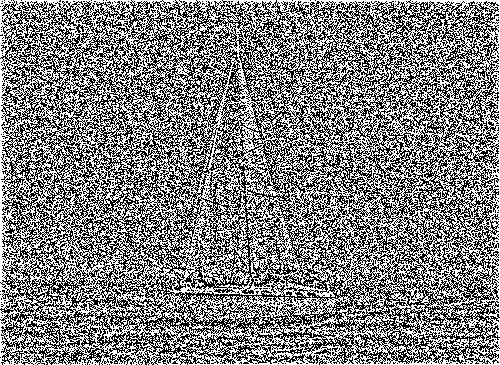
\includegraphics[width=\textwidth]{sail_sb_diff}
\caption{Split-Bregman}
\label{sail:sb:diff}
\end{subfigure}
\caption{Diff of each result with the noisy image, (a) shows the result of a standard Gaussian blur denoising using a width of 4.}
\label{fig:sailboat:diff}
\end{figure}




\subsection{Primal-Dual Algorithm}

The Primal-Dual algorithm is very fast.
As Figure \ref{fig:timing} shows, its averaged runtime was under a second.
It is very comparable to Split-Bregman and they only differed by a few tenths of a second.
It would be interesting to see how they compare on some larger images, unfortunately time limitations don't allow for investigating that further right now.

Primal-Dual also had very good quality results.
As mentioned before, it is somewhat difficulat to choose a "best" quality image from those shown.
For example Figures \ref{camera:pd},\ref{camera:pd:diff} show the result of running Primal-Dual on the camera man image.
As you can see the denoised images looks good.
The difference images shows that we probably coud have stopped the iterations a little sooner, as the edges seem to be smoothed more than the other algorithms.
Perhaps using a quantitative stopping criteria could have helped in that regard.

Numerically Primal-Dual was better behaved than Chambolles - it wasn't quite as hard to choose some parameters to make the algorithm work.

I chose $\lambda=0.0415$.  
The Primal-Dual paper suggested a way of estimating $\lambda$, but instead I've just used one of the values they reported, which seems to have performed fine.
I chose the initial $\tau=0.2$, where $\tau$ and $\theta$ were updated each time step using the the following formulas:
\begin{align*}
\tau &= 0.2 + k*0.08
\theta &= (0.5 + 5/(15+k))/\tau
\end{align*}

where $k$ is the iteration.
These choices seem to perform fine on the test images used.

\begin{figure}
\centering
\graphicspath{{images/}}
\begin{subfigure}[b]{0.4\textwidth}
\centering
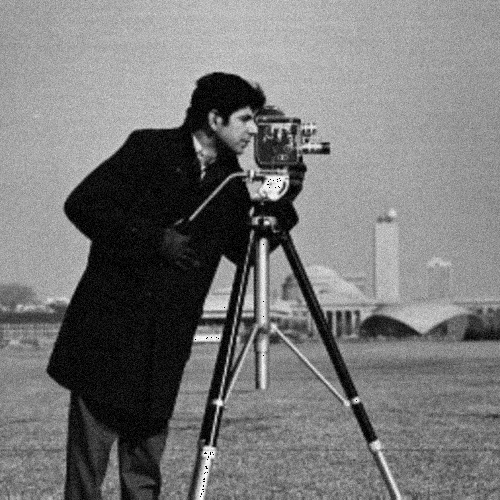
\includegraphics[width=\textwidth]{cameraman_10}
\caption{Noisy}
\label{camera:noise}
\end{subfigure}
\begin{subfigure}[b]{0.4\textwidth}
\centering
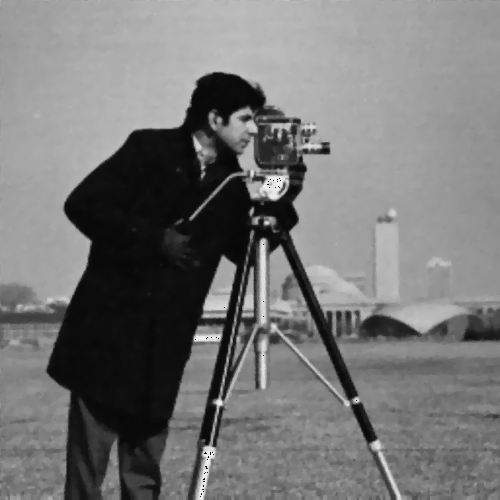
\includegraphics[width=\textwidth]{cameraman_10_ch}
\caption{Chambolle's}
\label{camera:ch}
\end{subfigure}
\begin{subfigure}[b]{0.4\textwidth}
\centering
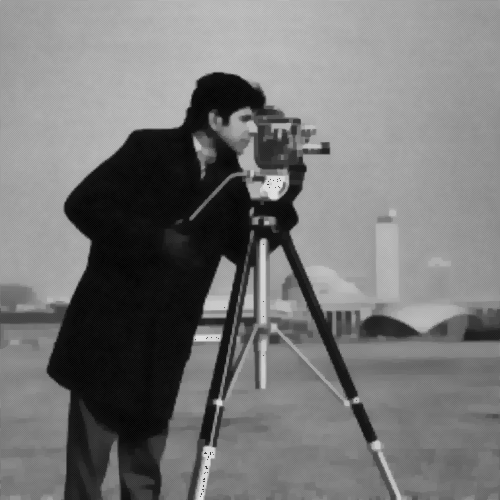
\includegraphics[width=\textwidth]{cameraman_10_pd}
\caption{Primal-Dual}
\label{camera:pd}
\end{subfigure}
\begin{subfigure}[b]{0.4\textwidth}
\centering
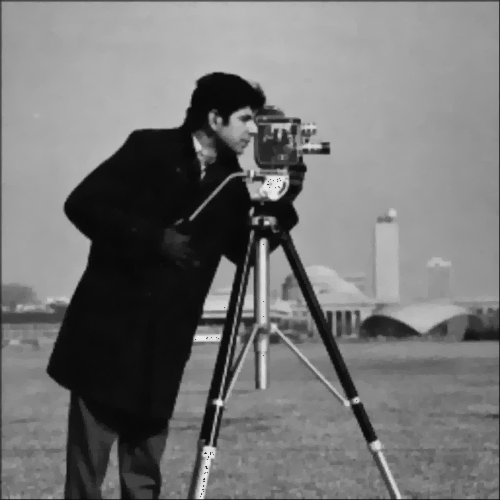
\includegraphics[width=\textwidth]{cameraman_10_sb}
\caption{Split-Bregman}
\label{camera:sb}
\end{subfigure}
\caption{Results of each algorithm on a noisy image of a cameraman.}
\label{fig:cameraman:dn}
\end{figure}

\begin{figure}
\centering
\graphicspath{{images/}}
\begin{subfigure}[b]{0.4\textwidth}
\centering
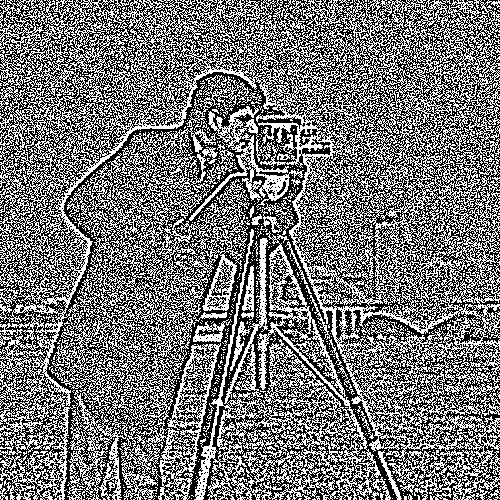
\includegraphics[width=\textwidth]{camera_blur_diff}
\caption{Gaussian blur}
\label{camera:gauss:diff}
\end{subfigure}
\begin{subfigure}[b]{0.4\textwidth}
\centering
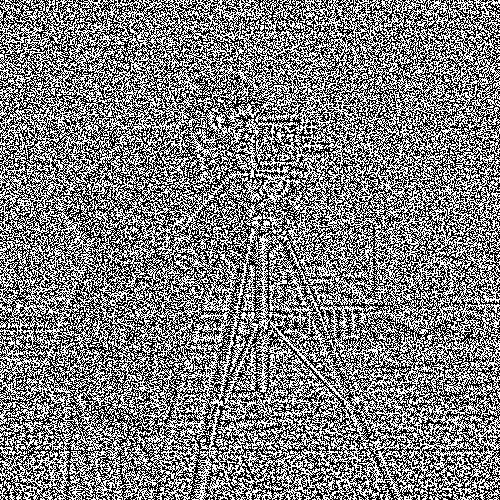
\includegraphics[width=\textwidth]{camera_ch_diff}
\caption{Chambolle's}
\label{camera:ch:diff}
\end{subfigure}
\begin{subfigure}[b]{0.4\textwidth}
\centering
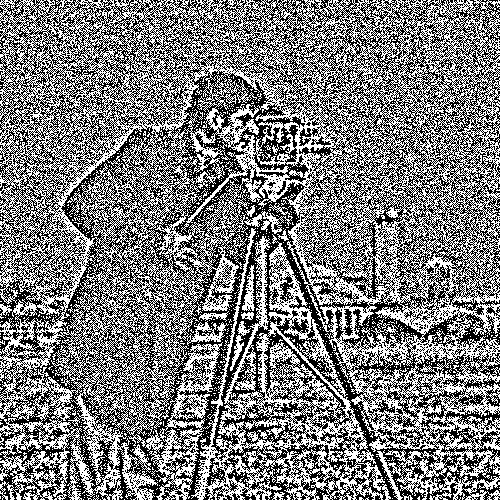
\includegraphics[width=\textwidth]{camera_pd_diff}
\caption{Primal-Dual}
\label{camera:pd:diff}
\end{subfigure}
\begin{subfigure}[b]{0.4\textwidth}
\centering
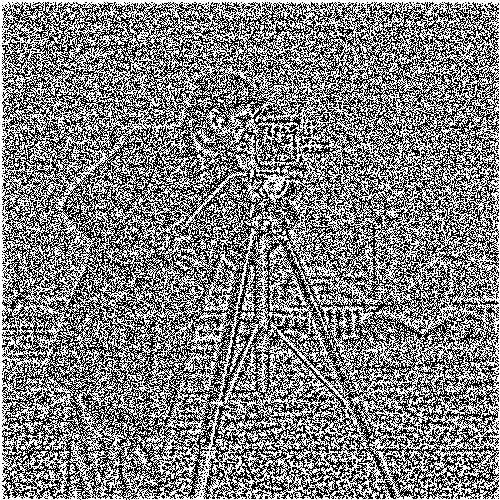
\includegraphics[width=\textwidth]{camera_sb_diff}
\caption{Split-Bregman}
\label{camera:sb:diff}
\end{subfigure}
\caption{Diff of each result with the noisy image, (a) shows the result of a standard Gaussian blur denoising using a width of 4.}
\label{fig:cameraman:diff}
\end{figure}

\subsection{Split-Bregman Algorithm}

Split-Bregman was the fastest algorithm, again shown in Figure \cite{fig:timing}.
As mentioned previously, this algorithm slightly outperformed Primal-Dual by a few tenths of a second.

The quality of Split-Bregman is very good, which is very exciting for such a fast algorithm!

Another very appealing feature Split-Bregman is it's simplicity and Numerical tolerance. 
I chose $\mu=0.1$ without any prior information and the algorithm converged very quickly.
It was surprising how forgiving and quick the algorithm is.

It's important to note that for this project I only implemented the Anisotropic Split-Bregman.
In the future it would be of interested ot compare the isotropic version as well.

Even though this is the anistropic version, the results don't appear very different from the Primal-Dual and Chambolle's isotropic solutions.

Looking at Figure \ref{slice:sb}, you can see the result of Split-Bregman on a slice of seismic sensor data.
Looking at the data, one can see that it might be of interested to a geologist or geophysicist to see the specific horizons in the data.
To that end the image was first histogram equalized to bring out the contrast.
However with the constrast also emphasizes some of the discontinuities in the horizons.

I was curious to see how the total variation denoising performed on the data.
The results appear encouraging. 
There doesn't appear to be any bad blurring across edges, and the roughness of the original equalized image appears to be smoothed out.
A more detailed analysis shows that there are some blurring of the data, especially in regions where the lines are more unclear.
It would be interesting to see how the algorithm performs on the volume data directly.


\begin{figure}
\centering
\graphicspath{{images/}}
\begin{subfigure}[b]{0.5\textwidth}
\centering
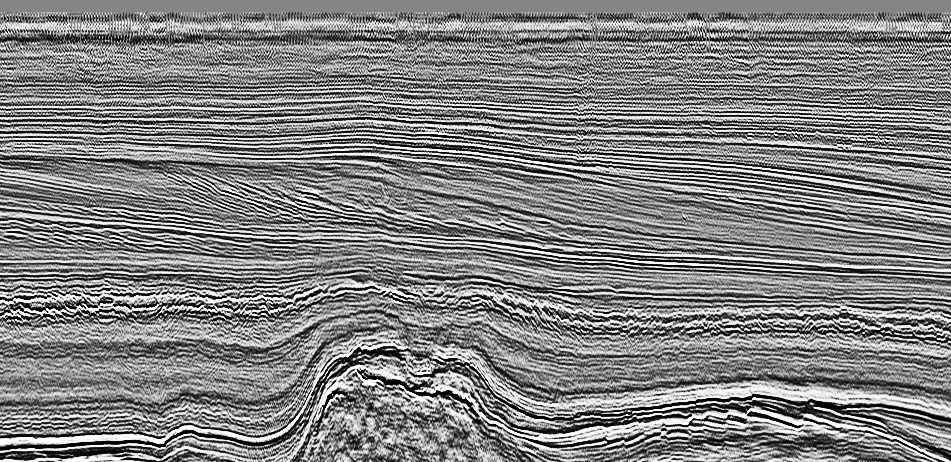
\includegraphics[width=\textwidth]{slice_eq}
\caption{Equalized no denoising}
\label{slice:noise}
\end{subfigure}
\begin{subfigure}[b]{0.5\textwidth}
\centering
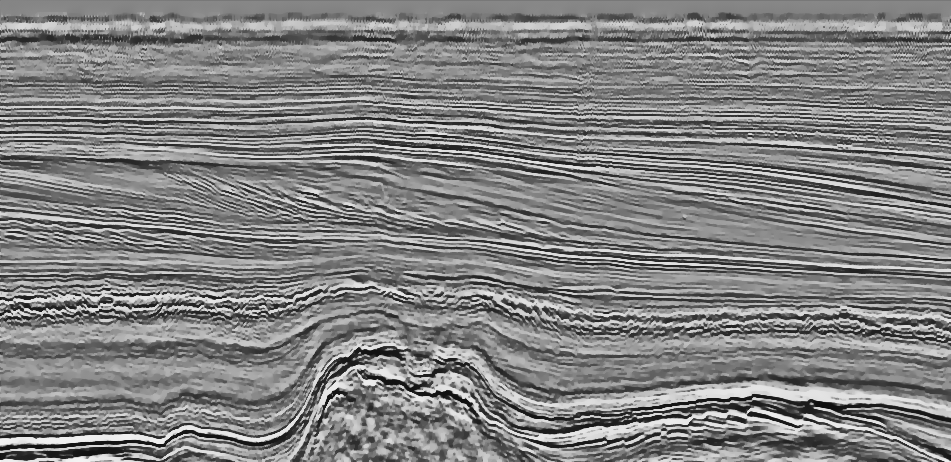
\includegraphics[width=\textwidth]{slice_eq_ch}
\caption{Chambolle's}
\label{slice:ch}
\end{subfigure}
\begin{subfigure}[b]{0.5\textwidth}
\centering
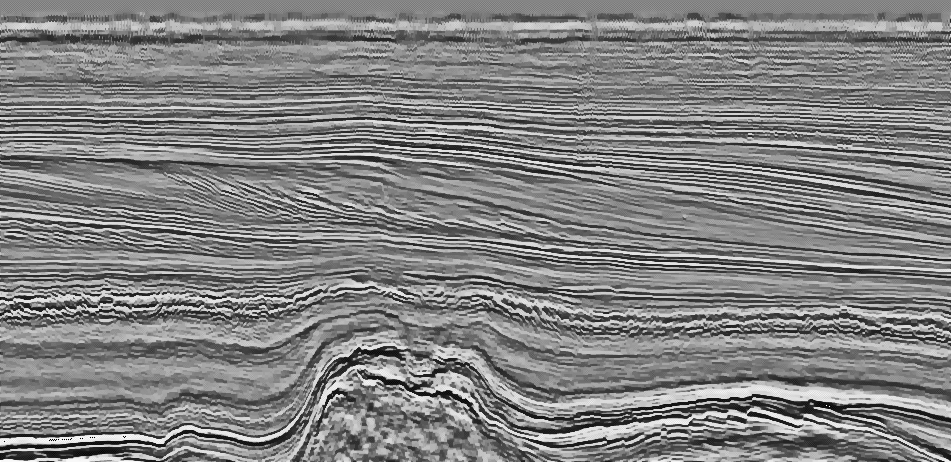
\includegraphics[width=\textwidth]{slice_eq_pd}
\caption{Primal-Dual}
\label{slice:pd}
\end{subfigure}
\begin{subfigure}[b]{0.5\textwidth}
\centering
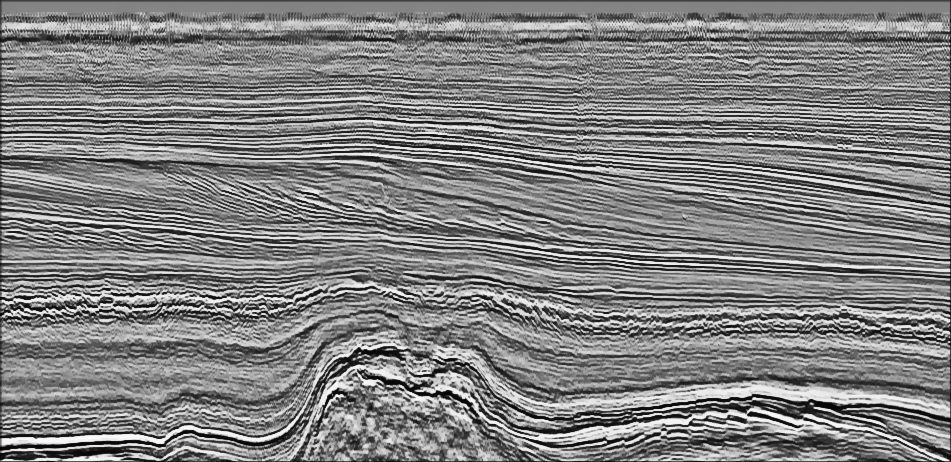
\includegraphics[width=\textwidth]{slice_eq_sb}
\caption{Split-Bregman}
\label{slice:sb}
\end{subfigure}
\caption{Results of each algorithm on a slice of a seismic volume from the OpendTect project \cite{opendTectWeb}. The slice has been equalized prior to smoothing to enhance appearance of horizons.}
\label{fig:slice:dn}
\end{figure}


\section{Conclusion}

This was a very interesting project.
It was very enlightening to learn first hand some of the problems and strengths of the different algorithms.
From class discussions and reading the papers, I knew that Primal-Dual was faster than Chambolle's but I didn't realize how drastic the improvement was.
Additionally it's interesting to see how robust and fast Split-Bregman is.
It's a shame I don't have time to pursue the topics deeper, it would have been interesting to continue comparing across different measurements, and especially to incorporate other non-linear methods like Perona-Malik and the Isotropic Split-Bregman.

\begin{figure}
\centering
\graphicspath{{../images/}}
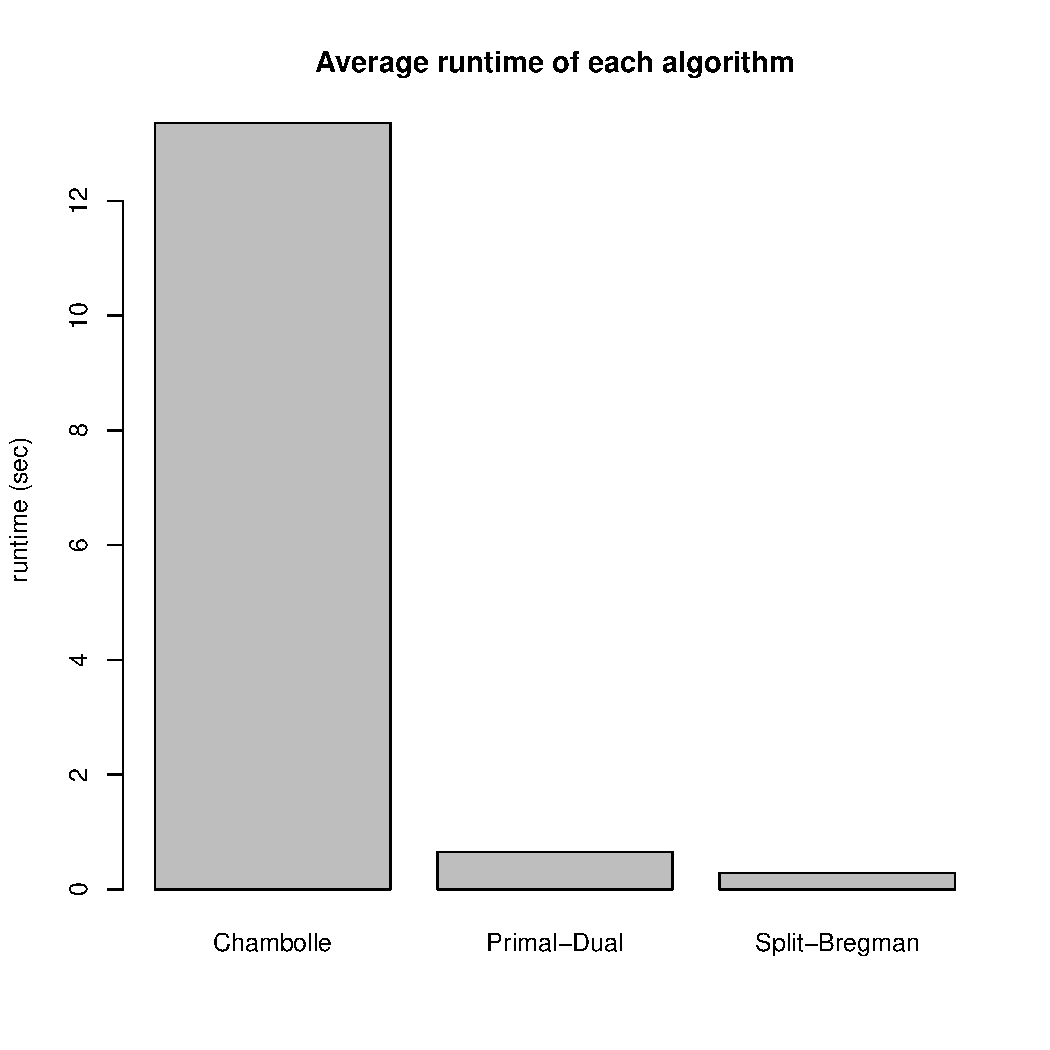
\includegraphics[width=0.5\textwidth]{average_timing}
\caption{Average time spent accross all images by algorithm.  Used visual stopping criteria.}
\label{fig:timing}
\end{figure}



\bibliography{nonlinear_smoothing}

\end{document}
